\documentclass[../Languages.tex]{subfiles}

\begin{document}
\usec{C\#}\label{sec:c_}

\texttt{C\#} is a multi-paradigm programming language encompassing strong
typing, imperative, declarative, functional, generic, object-oriented
(class-based), and component-oriented programming disciplines. It was developed
by Microsoft within it \textbf{.NET} initiative and later approved as a
standard by Ecma (ECMA-334) and ISO (ISO/IEC 23270:2006). \texttt{C\#} is one
of the programming languages designed for the Common Language Infrastructure.

\texttt{C\#} is a general-purpous, object-oriented programming language. Its
development team is lead by Anders Hejlsberg. The most recent verseion is
\texttt{C\# 7.2}, which was released in 2017 along with Visual Studio 2017
version 15.5.

\subsection{Influence}\label{sub:influence}

\begin{Figure}
  \centering
  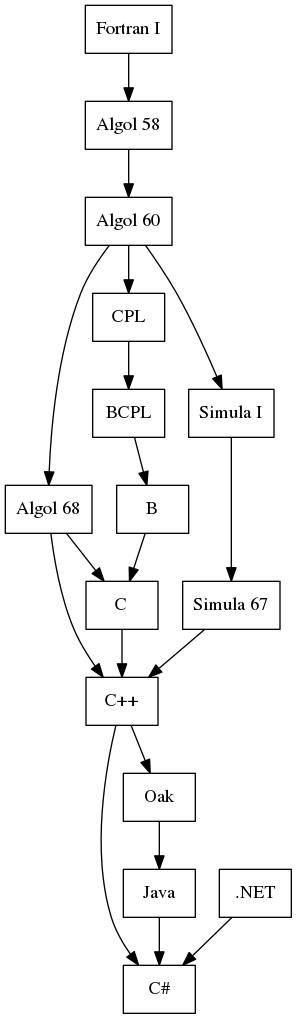
\includegraphics[height=0.5\textheight]{csharp}
  \captionof{figure}{Inheritance diagram for \cd{C\#}.}
\end{Figure}

\newpage
\end{document}
